\documentclass[letterpaper,11pt]{article}
\setlength{\textwidth}{6.5in}
\setlength{\hoffset}{0in}
%TODO: tweak these a bit more
\setlength{\voffset}{-0.5in}
\setlength{\textheight}{8.75in}
\setlength{\marginparsep}{0in}
\setlength{\marginparwidth}{0in}
\setlength{\oddsidemargin}{0in}

\usepackage{aas_macros}
\usepackage{amssymb}
\usepackage{caption}
\usepackage{hyperref}
\usepackage{listings}
\usepackage{mathabx}
\usepackage{setspace}
\doublespacing
\usepackage{siunitx}
\DeclareSIUnit\solarradius{R_\Sun}
\DeclareSIUnit\solarmass{M_\Sun}
\usepackage{subcaption}
\usepackage{tabularx}


\usepackage{graphicx}
\usepackage{lineno}
\usepackage[authoryear,square,colon]{natbib}
\bibpunct{[}{]}{;}{a}{,}{,~}

\usepackage{lipsum}

\begin{document}


\title{Searching for the $E^{-3/2}$ Suprathermal Power Law Tail in Parker Solar Probe's IS$\Sun$IS Data}
\author{A. Merrill}
\date{\today}
\maketitle

%\linenumbers

\begin{abstract}
The  \textit{Advanced  Composition  Explorer} (ACE)  and  the  \textit{Ulysses}  spacecraft revealed the presence of a common power-law spectrum of ions in the solar wind, the shape of which is independent of solar activity.  The highest energy particles in this distribution are a direct interest to human affairs as they can serve as the seed population for large, destructive events that can harm ground- and air-based equipment.  The mechanisms that create this common distribution are unknown, but by studying the behavior of the spectrum  at  closer  radii  more  can  be  learned  about  their  origin.  Furthermore, this relationship is altogether poorly studied within \SI{1}{\astronomicalunit}.  I investigate the first year and a half of Parker Solar Probe's data to find evidence of this spectrum in this previously unstudied region. I find weak evidence to suggest the existence of a common spectrum of protons from 60 to \SI{200}{\kilo\electronvolt} inside the region being studied.  Further work is required to uncover the phenomena  in  this  region  that  determine  the  shape  of  the  solar  wind spectra.
\end{abstract}



\section{Introduction}
\label{sec:intro}
The solar wind in regions above \SI{0.3}{\astronomicalunit} has been studied directly~\citep{McComas2007}, and a considerable understanding of the population of solar wind particles and their distributions has been gained about these regions~\citep{Fisk2012,Fisk2006,Fisk2008,Gloeckler2000}.  One particular phenomenon that our current understanding of accelerating processes in the solar wind fails to explain is the existence of an omnipresent power law spectrum of solar wind speed with a spectral index of $-5$; alternatively, this can be expressed as a power law of particle energy with spectral index of $-{3 \over 2}$~\citep{Fisk2012}.

\subsection{Acceleration of Solar Energetic Particles}
There are two known mechanisms that accelerate solar energetic particles (SEPs) that are capable of working over a broad spectrum of energies (a few \si{\kilo\electronvolt} to \si{\giga\electronvolt}).  \textit{Implusive} SEPs can result from magnetic-reconnection driven processes occurring during solar flares.  \textit{Gradual} SEP events can be created from coronal mass ejection-driven shocks~\citep{Desai2016}.  

A seed population of suprathermal particles (ie., \SI{>10}{\kilo\electronvolt}) is responsible for the acceleration of most solar energetic particles (SEPs), rather than the bulk solar wind~\citep{Mewaldt2012}.  The seed population for SEP events is of particular interest to human affairs as large SEP events can cause significant harm to humans and machinery in space and, in extreme circumstances, even those on the ground~\citep{Desai2016}.  This seed population is directly concerned with the power law spectrum seen in the solar wind as the seed population for SEP events is composed of suprathermal ions, the amount of which is dictated by the power law spectrum.  I search for the existence of this spectrum of ions in the solar wind in regions below \SI{0.3}{\astronomicalunit}.

\subsection{Instrumentation}
\label{sec:intro:instrumentation}
Parker Solar Probe (PSP) provides a previously unseen view of the solar wind inside Earth's orbit.  Diving from more than 60 to less than \SI{10}{\solarradius}, the spacecraft plunges into the solar corona to observe the phenomena that accelerate the solar wind and inflate the heliosphere.  In particular, PSP's closer view of the Sun can help explain how the corona is heated and how this power law spectrum is created in the solar wind~\citep{McComas2014,McComas2007}.

I use data from PSP's IS$\Sun$IS EPI-Lo instrument to look for the existence of the common power law tail in these regions close to the Sun.  EPI-Lo is a time-of-flight based mass-spectrometer capable of measuring ions and electrons varying from approximately \SI{20}{\kilo\electronvolt} to \SI{5}{\mega\electronvolt}.  Of interest here are EPI-Lo's specific capabilities surrounding protons, for which the instrument is capable of measuring between 0.04 and \SI{7}{\mega\electronvolt}~\citep{McComas2014}.  EPI-Lo is made of eight \SI{45}{\degree} wedge segments, each of which has 10 entrances for particles to strike a solid state detector.

%\subsection{Layers of Protection for the Earth}
%The planets are protected from galactic cosmic radiation by the ever-flowing solar wind that inflates the heliosphere.  

%The Parker Solar Probe is uniquely positioned to observe the origin of the solar wind.  

\section{Analysis}
\label{sec:analysis}
At the time of beginning the analysis, data from the beginning of PSP's flight (end of September 2019) through early January 2020 were available.  Events were selected by plotting a spectrogram of hourly- and directionally-averaged time-of-flight high energy resolution proton fluxes (Channel T Flux in the IS$\Sun$IS EPI-Lo Level 2 dataproducts) against time and energy for the entire duration of time for which data was available.  Fifteen events were found in PSP's data during this time.  The spectrogram from which events were selected is shown in Figure \ref{fig:flux_global}.

\begin{figure}[htbp]
\centering
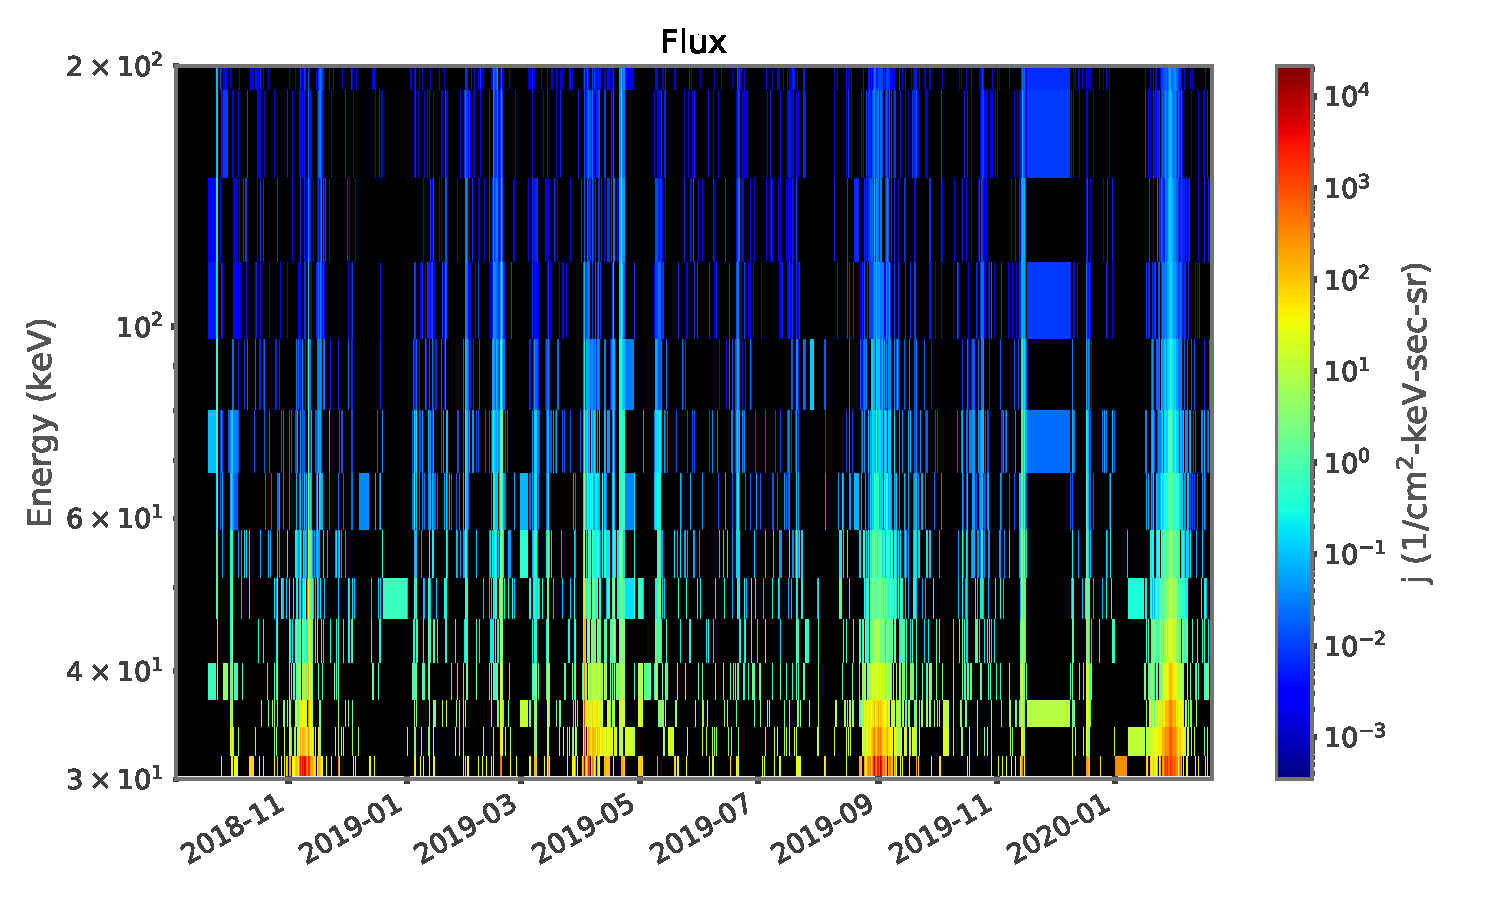
\includegraphics[width=1.\linewidth]{figures/flux_global(notshown).pdf}
\caption{Flux (j) versus energy and time for the duration of the mission at the time data analysis was started.  Individual events generally lasted for the approximate duration of a few days, making them too small to indicate on the spectrogram.  Notice that solar encounters are visible occurring approximately every 5 months starting in November 2018.}
\label{fig:flux_global}
\end{figure}


% TODO: Use np_array_to_latex to automate this table construction.
%Events identified are shown in Table \ref{tab:events}.
%
%\begin{tabularx}{\textwidth}{c | c | c | c  | X}
%Event number & Start time & Stop time & r & Eqn. \ref{eqn:flux} exponent \\
%\hline
%00 & 2018-09-25 & 2018-09-25 & radiusasdf & someoate \\
%01 & 2018-11-11 & 2018-11-12 & radiusasdf & someoate \\
%02 & 2018-11-15 & 2018-11-19 & radiusasdf & someoate \\
%03 & 2019-01-31 & 2019-02-01 & radiusasdf & someoate \\
%04 & 2019-02-13 & 2019-02-18 & radiusasdf & someoate \\
%05 & 2019-02-18 & 2019-02-19 & radiusasdf & someoate \\
%06 & 2019-03-06 & 2019-03-08 & radiusasdf & someoate \\
%07 & 2019-03-13 & 2019-03-15 & radiusasdf & someoate \\
%08 & 2019-04-02 & 2019-04-03 & radiusasdf & someoate \\
%09 & 2019-04-04 & 2019-04-04 & radiusasdf & someoate \\
%10 & 2019-04-17 & 2019-04-18 & radiusasdf & someoate \\
%11 & 2019-04-20 & 2019-04-23 & radiusasdf & someoate \\
%12 & 2019-06-19 & 2019-06-21 & radiusasdf & someoate \\
%13 & 2019-10-22 & 2019-10-26 & radiusasdf & someoate \\
%14 & 2019-11-13 & 2019-11-16 & radiusasdf & someoate \\
%\\
%\end{tabularx}

\citet{Fisk2006} suggest a model of compressional acceleration in solar wind turbulence that predicts a functional dependence of flux on energy in the suprathermal tail as
\begin{equation}
j = j_0 T^{-3 \over 2}.
\label{eqn:flux}
\end{equation}
I attempt to recover this model from fits to the spectra of each event.

The first approach to find evidence of the model in Equation \ref{eqn:flux} fitting the spectra of the events was to simply apply a fit to the data between 40 and \SI{160}{\kilo\electronvolt} of an event-duration- and directionally-averaged spectrum of each event.  This energy region was determined by visual inspection of the events to to fit the region most like a power-law inside the suprathermal region described by \citet{Fisk2008}. This yielded fits like those shown in Figure \ref{fig:naive_fits}.  The exponents fit to these spectra did not well match to the expected $-{3 \over 2}$.

\begin{figure}
\centering
\begin{subfigure}{.45\textwidth}
\centering
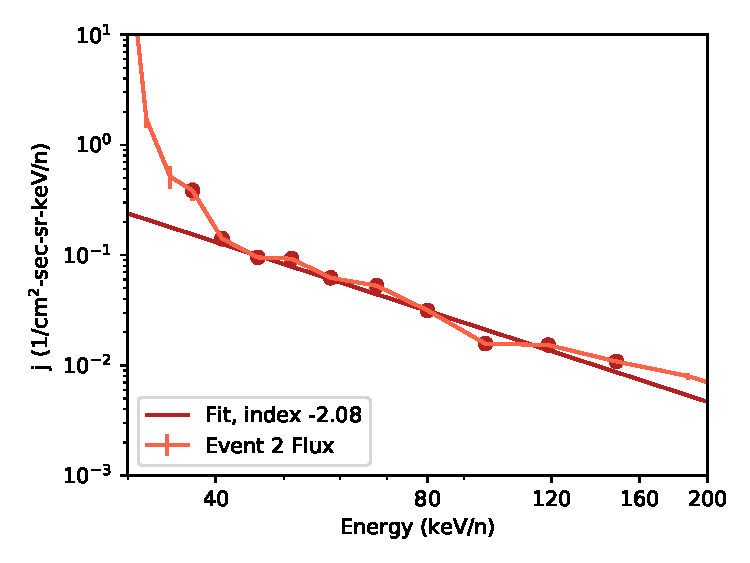
\includegraphics[width=1.\linewidth]{figures/spectrum_02.pdf}
\caption{Event 02.  Exponent of -6.97.}
\end{subfigure}
\begin{subfigure}{.45\textwidth}
\centering
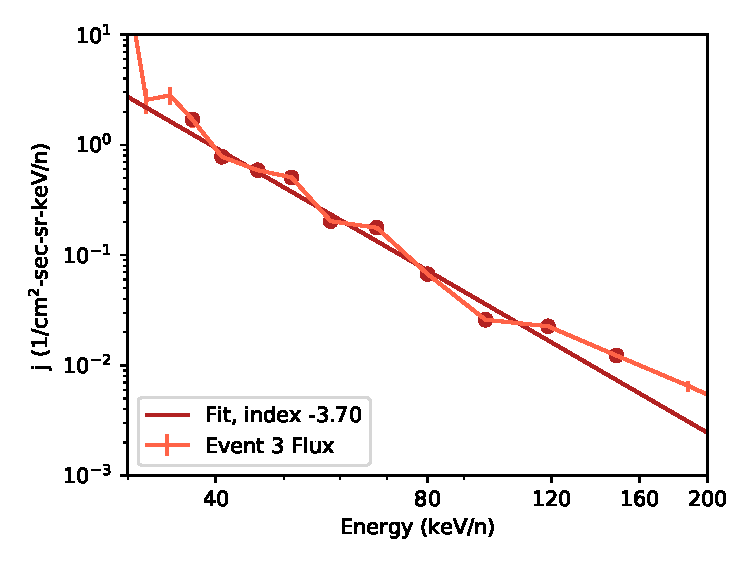
\includegraphics[width=1.\linewidth]{figures/spectrum_03.pdf}
\caption{Event 03.  Exponent of -6.74.}
\end{subfigure}
\caption{Fits of the spectra from Events 02 and 03.}
\label{fig:naive_fits}
\end{figure}



\section{Discussion}
\label{sec:discussion}



\section{Conclusion}
\label{sec:conclusion}

\section{Acknowledgments}
Special thanks to Dana Filoti and James Ryan for their questions during the URC.



%\bibliographystyle{thesis}
\bibliographystyle{abbrv}
\bibliography{thesis}

\end{document}
